\documentclass[12pt]{article}
%Gummi|065|=)
\usepackage{amsmath, amsfonts, amssymb}
\usepackage[margin=0.5in]{geometry}
\usepackage{xcolor}
%\usepackage{graphicx}
%\usepackage{graphicx}
\newcommand{\off}[1]{}
\DeclareMathSizes{20}{30}{21}{18}

\newcommand{\myhrule}{}

\newcommand{\two }{\sqrt[3]{2}}
\newcommand{\four}{\sqrt[3]{4}}

\newcommand{\dash}{
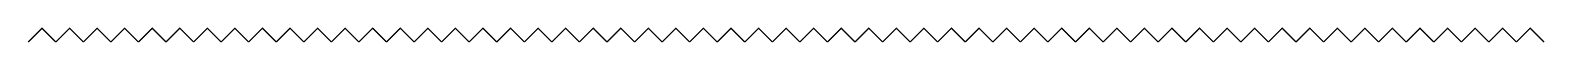
\begin{tikzpicture}[scale=0.35]
\foreach \x in {1,...,55}{
	\draw (\x,-0.25)--(\x+0.5,0.25)--(\x+1,-0.25);
}
\end{tikzpicture}
}

\newcommand{\sq}[3]{
\node at (#1+0.5,#2+0.5) {#3};
\draw (#1+0,#2+0)--(#1+1,#2+0)--(#1+1,#2+1)--(#1+0,#2+1)--cycle;
}

\usepackage{tikz}

\title{\textbf{Prime Number Theorem}}
\author{John D Mangual}
\date{}
\begin{document}

\fontfamily{qag}\selectfont \fontsize{25}{30}\selectfont

\maketitle

\noindent The Wiener-Ikehera Tauberian Theorem implies the Prime Number Theorem, as can be shown in various places. \\ \\ None of those discussions really explain to me:
\begin{itemize}
\item connection to divergent series
\item how we can proceed on our own
\end{itemize}
Norber Weiner's original argument is very easy to follow:
M\"{o}bius inversion is what gives the series to start:
$$ \sum_{m=1}^\infty x^m \log m = \sum_{n=1}^\infty \Lambda(n) \frac{x^n}{1-x^n} $$
and then set $x = e^{-\xi}$ and $\xi \to 0$ (or $x \to 1$). \newpage

\noindent
The two limiting behaviors are rather diffrent
$$  \frac{x^n}{1 - x^n}  = \left\{  \begin{array}{rl}
1/n\epsilon & \text{ as }x \to 1 \\
\epsilon^n & \text{ as } x \to 0 \end{array}\right. $$
and the cuttoff point is when $(1 - \epsilon)^n$ is getting small (near $n = 1/\epsilon$)
$$ \sum_{n=1}^\infty \Lambda(n) \frac{\xi e^{-n\xi}}{1-e^{-n\xi}} \approx \sum_{n=1}^{1/\xi} \frac{\Lambda(n)}{n} $$
Maybe if we take the derivative of both sides:
$$  \sum_{n=1}^\infty \Lambda(n) \; \frac{d}{d(n\xi)}\bigg[ \frac{n\xi }{1-e^{n\xi}} \bigg]  \approx \sum_{n=1}^{1/\xi} \Lambda(n) $$
 And clearly the two sides are approximate so we are done.
$$ \frac{d}{du} \left( \frac{u}{1 - e^u} \right) = \left\{  \begin{array}{cl}
1 & \text{ as }u \to 0 \\
ue^{-u} & \text{ as } u \to \infty \end{array}\right. $$
The left side can be shown to be 1 through ``elementary" arguments. 
$$  \sum_{n=1}^\infty \Lambda(n) \; \frac{d}{d(n\xi)}\bigg[ \frac{n\xi }{1-e^{n\xi}} \bigg] \approx \frac{1}{\xi} + O(\log \xi)$$

\newpage

\fontfamily{qag}\selectfont \fontsize{12}{10}\selectfont


\begin{thebibliography}{}

\item David Vernon Widder \textbf{The Laplace Transform} Princeton University Press, 1948.

\item Norbert Wiener \textbf{Tauberian Theorems} Annals of Mathematics Vol. 33, No. 1 , pp. 1-100

\item G. H. Hardy \textbf{Divergent Series} Oxford University Press 1973





\end{thebibliography}



\end{document}